\documentclass[pdftex,10pt,a4paper,oneside]{article}
%Can change the pt, papersize etc.

\usepackage{algorithm}
\usepackage{algorithmic} %Algorithm styles, need to be nested for the example shown
\usepackage{fancyhdr} %For our headers
\usepackage{graphicx} %Inserting images
\usepackage{lipsum}  %Blank text fill, delete me when finished
\usepackage{setspace} %Spacing on the front page for crest and titles
\usepackage[]{fncychap} % Styles can be Sonny, Lenny, Glenn, Conny, Rejne, Bjarne and Bjornstrup
\usepackage[hyphens]{url} %Deals with hyphens in urls to make them clickable
\usepackage{xcolor} %Great if you want coloured text
\usepackage{tabularx}
\usepackage{appendix} %Take a wild guess slick

%KEEP THIS ONE LAST it's quite buggy, it allows you to click on links within the pdf and web links without changing the colour. The mouse cursor simply changes its icon to indicate to the user. Great tool - still awkward
\usepackage[hidelinks]{hyperref}


%This will tell the compiler to do the header style, page and spacing between the header and text
\fancyhf{}
\renewcommand{\headrulewidth}{0.2pt}

\begin{document}

\begin{spacing}{2}
	\begin{center}
		
\includegraphics[scale = 0.20]{ASU.png}
	\end{center}
	\vspace{5mm}
	\begin{center}
		\textbf{\begin{LARGE}
	        Assigment 4
		\end{LARGE}}
		\vspace{5mm}
	\end{center}
	\begin{center}
		\textbf{\large Mohamed Yasser Ahmed Hanafy Elesaily\\ code: 1601287}
		\vspace{10mm}
	\end{center}
	\begin{center}
	     {\large Supervisor: Dr. Gamal Ibrahim }\\
		\textbf{\large Department of Computer Systems Engineering}\\
		{\large Faculty of Engineering at Ain Shams University}\\
		{\large January 2020\\}
	\end{center}
\end{spacing}

\pagebreak

\tableofcontents

\pagebreak

\section{Introduction}
We use MPI library for c to calculate $\pi$ using numerical formula
$$ \pi = \sum_{i = 0}^\infty \frac{(i!)^2 2^{i+1}}{(2i + 1)!} $$
MPI is used in distributed systems to communicate with each other. No need for shared memory but they use message between the system. 

\section{Process and Communication}
I divide my process into one master process that collect the data and several process each one calculate his iteration then send the result into master node (see figure \ref{s}).
\begin{figure}[H]
  \centering
  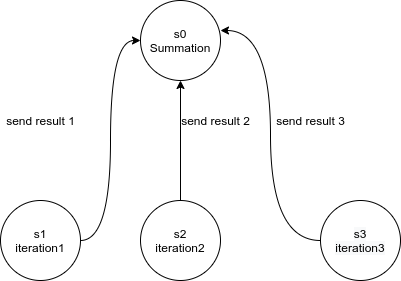
\includegraphics[width=100mm,scale=5]{m.png}
  \caption{Communication between nodes}
  \label{s}

\end{figure}
but we firstly get input from the user about the limit of $i$ in the equation. we can get input
from the user from process 0 only ($s0$) so we should recive it to each process (see figure \ref{a})
\begin{figure}[H]
  \centering
  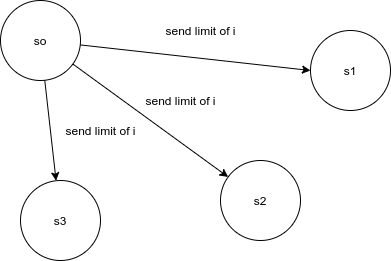
\includegraphics[width=100mm,scale=5]{s (1).png}
  \caption{processes receive the limit of i}
  \label{a}

\end{figure}
\section{Result}
\begin{figure}[H]
  \centering
  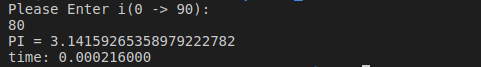
\includegraphics[width=100mm,scale=5]{image2.png}
  \caption{result of pi without using mpi}
  \label{a}

\end{figure}
\begin{figure}[H]
  \centering
  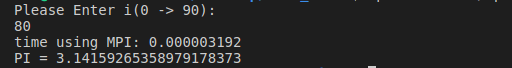
\includegraphics[width=100mm,scale=5]{image1.png}
  \caption{result of pi using mpi}
  \label{a}

\end{figure}
program that run using mpi is faster than the other program by $\%77$.
\end{document}
